\documentclass{article}
\usepackage{enumitem}
\usepackage{graphicx}
\usepackage{subcaption}
\usepackage{tikz}
\begin{document}

\begin{figure}[h]
	\centering
\begin{tikzpicture}
    % First figure
    \node[draw, rectangle, blue] (figure1) at (0,2) {\includegraphics[width=0.3\textwidth]{{"input_images 2.jpg"}};
    %\node[above=70pt, text width=3cm,align=center] at (figure1) {Input images};

    % Second figure
    \node[draw, rectangle, blue] (figure2) at (4,2) {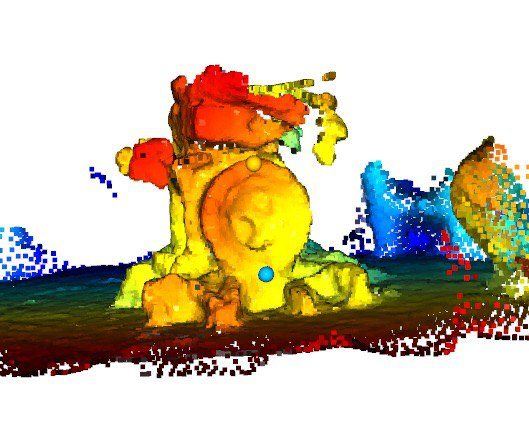
\includegraphics[width=0.25\textwidth]{"../3d_task_figure1/reference 2.jpg"}};
    %\node[above=70pt, text width=100pt,align=center] at (figure2) {Dense reconstruction Output};

    % Third figure
    \node[draw, rectangle, blue] (figure3) at (8,4) {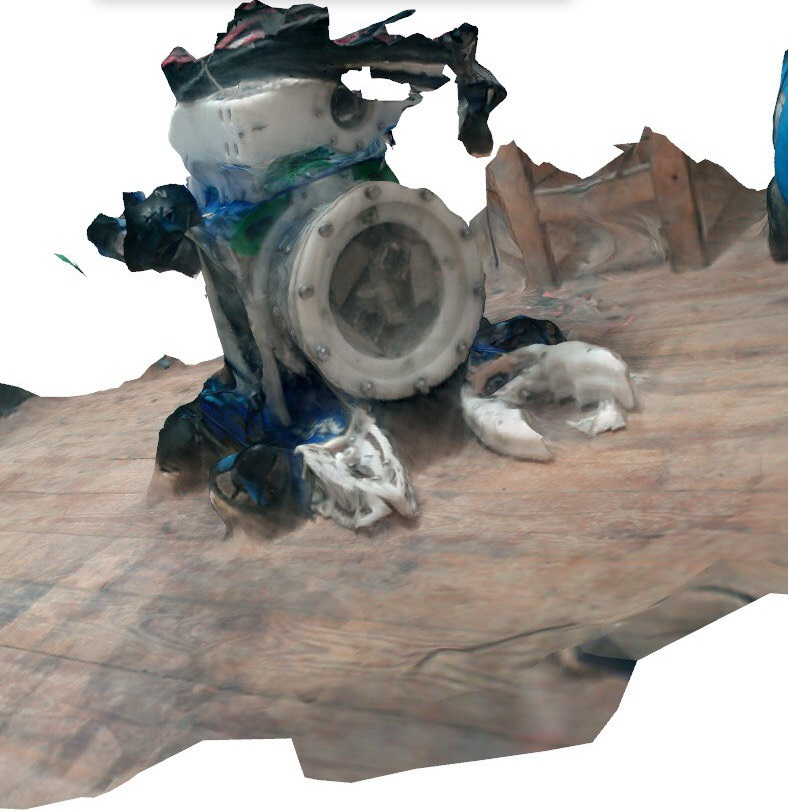
\includegraphics[width=0.27\textwidth]{op1.jpg}};
    %\node[above=70pt,text width=100pt,align=center] at (figure3) {Texture Output from different views};

    % third figure
    \node[draw, rectangle, blue] (figure4) at (8,0) {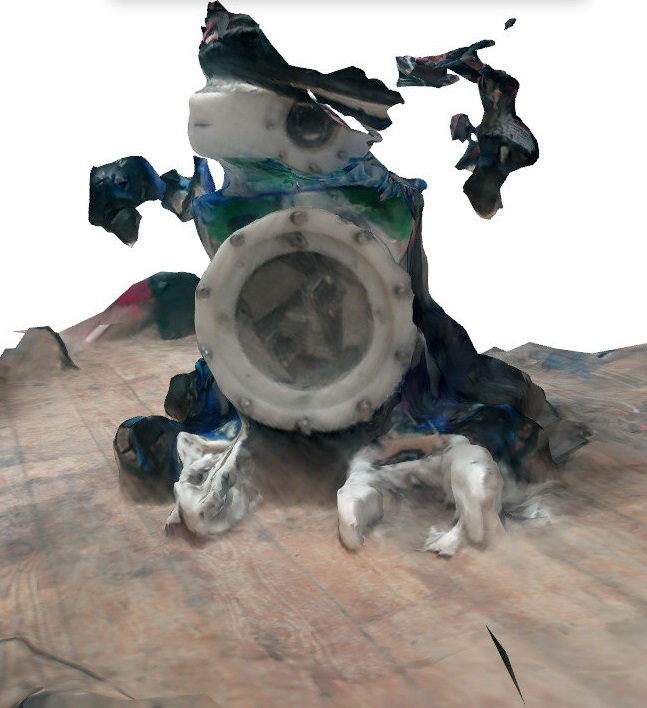
\includegraphics[width=0.27\textwidth]{op2.jpg}};
    
    % Arrow between figures
    \draw[->, line width=1.3pt, blue] (figure1) -- (figure2);
    \draw[->, line width=1.3pt, blue] (figure2) -- (figure3);
    \draw[->, line width=1.3pt, blue] (figure2) -- (figure4);

  \end{tikzpicture}
\caption{Reconstruction process}
\label{fig:reconstruction}
\end{figure}


\end{document}